% Report that introduces \MLEP
% Self-published, not peer-reviewed

\documentclass[11pt,letter]{article}
% Above is the standard document class.  If would like to use document
% class differently according to PDF or not, use the following:
% \RequirePackage{ifpdf}
% \ifpdf
% \documentclass[pdftex,. . . ]{. . . }
% \else
% \documentclass[. . . ]{. . . }
% \fi

\usepackage{fixltx2e}

%%%% PDF support
% Check if in PDF mode or not.  Usage: \ifpdf ... \else ... \fi
\usepackage{ifpdf}

\ifpdf
% microtype package for better typography with pdftex
\usepackage[protrusion=true,expansion=true]{microtype}
\fi


%%%% Geometry (paper size, margins, etc.)
% Change the size of body text and margins.  Refer geometry for more
% options.
%\usepackage[body={6.4in,9in}, top=1in, left=1in]{geometry}
% or simply use fullpage for a full page
\usepackage{fullpage}

\usepackage{parskip}
%\parskip=3mm   % Set the skip size between paragraphs


% The standard LaTeX font is Computer Modern. Other fonts are available.
%
% Other popular options are
% - Times:     \usepackage{mathptmx}
% - Palatino:  \usepackage{mathpazo}
% - New Century Schoolbook: \usepackage{newcent}
% - Another (better) Times: \usepackage{ntxtext}  % Times font
\usepackage{times}

\usepackage{xspace}

%%%% Math support (AMS math packages, symbols...)
% If you want to flush all equations to the left, or to set other
% options of amsmath, use the following line:
% \usepackage[fleqn]{amsmath}
\usepackage{amsmath}
% Uncomment line below to allow page break inside multi-line equations
% \interdisplaylinepenalty=2500

% Additional math packages
\usepackage{amsfonts,amssymb}
%\usepackage{bm} % for bold symbols like \bm{\alpha} or {\bm \alpha\beta}


%\usepackage{cases}  % Better than amsmath's cases environment


%%%% SI Unit support: should always use to typeset numeric data
% With option per-mode=symbol: kW/s, without it: kW s^{-1}
% Quick usage:
%   \num{1+-2i}
%   \num{.3e45}
%   \SI{number}{unit} or \si{unit}
% where unit is like:
%   kg.m.s^{-1} or \kilogram\metre\per\second
%   \si[per-mode=symbol]{\kilogram\metre\per\ampere\per\second} for
%        kg m / (A s)
%\usepackage[per-mode=symbol]{siunitx}


%%%% Graphic packages
% TODO: add more options/settings to this package
\usepackage{graphicx}
\ifpdf
\graphicspath{{figs/}{photos/}}
\else
\graphicspath{{figs/}{eps/}}
\fi

\usepackage{subfig}  % Sub-figures
% \usepackage{color}   % Support colors
\usepackage[svgnames, rgb]{xcolor}  % Support for color with standard names

% PGF/TikZ
%\usepackage{tikz}
%\usetikzlibrary{snakes,arrows,shapes,positioning}
% Some other TikZ libraries
% \usetikzlibrary{automata,calc,matrix}
% \usetikzlibrary{circuits.logic.US,circuits.ee.IEC}
% \usetikzlibrary{shapes.geometric,shapes.symbols,shapes.arrows}

% \usepackage{wrapfig}  $ Wrap text around figures

% \usepackage{vaucanson-g}  % Draw state machines


%%%% Special typesetting
% Algorithms
%\usepackage[ruled]{algorithm}    % For creating floating algorithms, in the algorithms bundle

% The followings are packages for creating actual algorithms
%\usepackage{algorithmic}  % Easy to use, Pascal-like, less flexible, in the algorithms bundle
%\usepackage{algorithm2e}  % More flexible, more like Pascal
%\usepackage{algpseudocode}  % In the algorithmicx package, flexible, more math-like

% For typesetting source code
%\usepackage{listings}


% Notes, comments
% \usepackage{todonotes}
% \usepackage{verbatim}   % better support for verbatims, comment environment

%%%% Customizations

% Customization of enumerate, itemize, description
%\usepackage{enumerate}  % Customize enumerate only
%\usepackage{enumitem}   % Customize enumerate, itemize, description


%%%% Set-up hyperref for hyperlinks, etc.
%%%% This should always come last in the preamble.

% The default \usepackage{hyperref} should work automatically.
% See hyperref for more options (visual, backlinks, etc.)
% Note that hyperref with pdftex seems fragile, especially with special symbols in section titles.
\ifpdf
  \usepackage[pdftex]{hyperref}
\else
  \usepackage[dvips]{hyperref}  % or dvipdfm
\fi

% CLEVER REFERENCES
% This package automatically infers the type of
% references (e.g. equations, figures, theorems, etc.) using the
% \cref* family of commands. If it is to be used, it should be loaded
% last. If hyperref and varioref is also used, the order should be
% varioref, hyperref, cleveref. To use with theorems correctly, either
% amsthm or ntheorem should be loaded, and all \newtheorem definitions
% must be placed AFTER the cleveref package is loaded. To use with a
% language other than English, the language should be set globally in
% the \documentclass command rather than solely in babel.

% \usepackage{cleveref} % Options: capitalise, noabbrev, nameinlink

% If using cleveref, all \newtheorem commands should be placed here.

%%%% BEGIN OF DOCUMENT
\title{\scshape \MLEP: a Matlab-EnergyPlus Co-simulation Interface}
\author{\textbf{Truong~X.~Nghiem}\\
Automatic Control Laboratory\\
Ecole Polytechnique F\'{e}d\'{e}rale de Lausanne (EPFL), Switzerland}
\date{}

\ifpdf
\pdfinfo{/Author (Truong X. Nghiem)
           /Title (MLE+: a Matlab-EnergyPlus Co-simulation Interface)
           /Keywords (matlab, energyplus, simulation, buildings)}
\fi

\newcommand{\MLEP}{MLE+\xspace}

\begin{document}
\maketitle

\tableofcontents{}

\section{Introduction}
\label{sec:introduction}

\MLEP is a Matlab toolbox for co-simulation with the whole-building
energy simulator \href{http://apps1.eere.energy.gov/buildings/energyplus/}{EnergyPlus}.  It is designed for engineers and researchers who are
familiar with Matlab and Simulink and want to use these software
tools in building energy simulation.  \MLEP is particularly useful for:
\begin{itemize}
\item Controller design: the energy simulation is carried out by
  EnergyPlus while the controller is designed and implemented in
  Matlab or Simulink.
\item Simulation and data collection: a large
  number of simulations, with different scenarios, can be carried out
  and their data is collected, stored and processed in Matlab.  The
  data can then be used for various purposes, e.g.\ for learning a
  model of the building system.
\item Simulation-based optimization: a
  non-linear optimizer, e.g.\ one in the Matlab's Global Optimization
  Toolbox, can be used to find optimal parameters or control sequences
  of the building system, by considering the building as a black-box
  whose execution is performed by simulations by EnergyPlus.
\end{itemize}

\MLEP toolbox provides a set of Matlab functions and classes, as well
as a Simulink library, for performing co-simulation with EnergyPlus.
The current version of \MLEP, as of \today{}, has been tested to work with EnergyPlus version 8.3.


\section{Comparison with BCVTB}
\label{sec:comparison-bcvtb}

\href{https://gaia.lbl.gov/bcvtb}{BCVTB} (Building Controls Virtual Test Bed) is a software environment for coupling different simulation programs for distributed simulation.
It is based on the Ptolemy II software environment and is developed at the Lawrence
Berkeley National Laboratory.

The co-simulation feature in EnergyPlus was originally developed for
BCVTB, however the communication protocol is open and can be used by
any program to perform co-simulation with EnergyPlus.  \MLEP is an
example of such programs.

Although Matlab / Simulink can be coupled with EnergyPlus via BCVTB, \textbf{its
full functionality cannot be used because it is only called by BCVTB
as a client}.
For example, interactive execution and debugging Matlab code are not
possible.
In fact, if the Matlab code or the Simulink model has an error, it is much more difficult to find and fix it with BCVTB than with \MLEP (which runs in the standard Matlab environment).
Furthermore, for users who mostly work with Matlab / Simulink and have never used Ptolemy, learning a new environment as Ptolemy is time-consuming and might not be worthwhile.

Advantages of BCVTB over \MLEP include:
\begin{itemize}
\item It is always up-to-date with the co-simulation feature in EnergyPlus.
\item It can be used to couple other programs besides EnergyPlus and
  Matlab / Simulink, such as Modelica and Radiance.  However, in the future, \MLEP will incorporate interfaces to these programs as well.
\item It is free, open-source and runs on Java.  Note that \MLEP is also
  free and open-source, but it requires Matlab / Simulink which are
  commercial.
\end{itemize}

Advantages of \MLEP over BCVTB include:
\begin{itemize}
\item It takes full advantage of the Matlab / Simulink environment,
  including interactive simulation, code debugging, low-level
  co-simulation API (Application Programming Interface), code
  generation, and all available toolboxes.  In other words, it
  integrates better with the Matlab / Simulink environment.
\item It is easier to extend \MLEP, using Matlab programming, for specialized
  applications and functions.  An example is large-scale optimization
  of building's design parameters using parallel simulations (with
  Matlab's Parallel Computing Toolbox and Distributed Computing
  Server).  Another example is a GUI for rapid development of building
  controllers, be it a simple PID controller or a complex Model
  Predictive Controller.
\item It is familiar to users who mainly use Matlab / Simulink, such as control engineers.
\end{itemize}

\section{Loose Coupling Co-simulation}
\label{sec:co-simulation}

\MLEP implements a \emph{loose coupling} co-simulation architecture between clients.
Generally speaking, each simulator performs its local simulation and exchange their variables only once at every fixed synchronization time step.
There is no iteration between clients at a time step or between any two consecutive time steps.
The readers are referred to \cite{hensen1999comparison,zhai2005performance,trcka2007comparison} for more details.

\section{Installation}
\label{sec:install}
\subsection{System Requirements}
\label{sec:install:requirements}

\begin{itemize}
\item \MLEP requires Matlab, and Simulink if you are going to use its Simulink library, of recent versions.  It has been tested in Matlab versions R2009b through R2015a.
\item Java must be enabled in Matlab.  Java socket library is used by \MLEP
for communication with EnergyPlus.
\item \href{http://apps1.eere.energy.gov/buildings/energyplus/}{EnergyPlus}: \MLEP should work well with the current version of EnergyPlus, which was version 8.3 at the time this report was last updated.
\item \href{https://gaia.lbl.gov/bcvtb}{BCVTB}.  \MLEP does not require BCVTB to run, however the ExternalInterface feature of EnergyPlus requires that BCVTB exists in the system.
\end{itemize}

\subsection{Install \MLEP}
\label{sec:install:installation}

After all system requirements of \MLEP are satisfied, installation of \MLEP is simple.
\begin{itemize}
\item First, download the compressed \MLEP distribution package and extract
it to a directory.  Let us call this directory \verb+<MLEPDir>+.
\item Start Matlab and add \verb+<MLEPDir>+ to the search path, either by the GUI
or by the following command: \verb+addpath(<MLEPDir>)+.
\item It is recommended to save the search path.
\end{itemize}

\section{\MLEP Usage}
\label{sec:usage}

\MLEP provides:
\begin{itemize}
\item A set of Matlab functions and classes for co-simulation with
EnergyPlus from Matlab code.  They all have prefix \emph{mlep}.
\item A library of Simulink blocks for co-simulation with EnergyPlus from
Simulink models.
\item Several utility functions.  They all have prefix \emph{mlep}.
\end{itemize}

\subsection{General configuration for co-simulation with EnergyPlus}
\label{sec-4-1}

In order to perform co-simulation with EnergyPlus, certain configurations
need to be done: the IDF model file may need to be instrumented to
allow importing and exporting variables from and to external programs,
and a configuration file named \emph{variables.cfg} needs to be created to
specify these input and output variables.  For more details, refer to
the \href{http://simulationresearch.lbl.gov/bcvtb/releases/latest/doc/manual/index.xhtml}{BCVTB manual} or the External Interface manual of EnergyPlus.

\subsection{The BCVTB protocol}
\label{sec-4-4}

A special protocol is used to exchange data between co-simulation
processes via sockets.  Each packet is a text string that contains a
sequence of numbers of the following format
\[ \begin{matrix}
  v & f & n_r & n_i & n_b & t & r_1 & r_2 & \cdots
\end{matrix} \]
where:
\begin{itemize}
\item $v$ is the version number (currently versions 1 and 2 are supported).
\item $f$ is a flag: 0 if normal, 1 if simulation stopped, negative if
error.
\item $n_{\text{r}}$, $n_{\text{i}}$, $n_{\text{b}}$ are the numbers of real variables, integer
variables, and Boolean variables respectively.  Currently, EnergyPlus requires that $n_{\text{i}}=0$ and $n_{\text{b}}=0$.
\item $t$ is the current simulation time in seconds.
\item $r_{\text{1}}$, $r_{\text{2}}$, \dots are the values of the variables, starting with real
ones, then integer ones, and finally Boolean ones.
\end{itemize}

For more details, refer to the \href{http://simulationresearch.lbl.gov/bcvtb/releases/latest/doc/manual/index.xhtml}{BCVTB manual}.

\subsection{Matlab functions and classes}
\label{sec-4-5}

Matlab functions in \MLEP can be classified into three groups:
\begin{itemize}
\item Start and stop co-simulation with EnergyPlus.
\item Send and receive data packets to and from EnergyPlus.
\item Encode and decode data packets.
\end{itemize}

This section only summarizes the functions and classes provided by
\MLEP.  Detailed information should be found by reading the help
text of the functions.

\subsubsection{Start and stop co-simulation}
\label{sec-4-5-1}

\begin{itemize}
\item To start a new co-simulation session, use the function
\verb+mlepCreate+.  Arguments include the path to the
EnergyPlus executable, its command-line arguments, the BCVTB
directory, and the host and port number for the communication
socket.  This function returns the status and the sockets created
for communication.
\item When the co-simulation terminates, the communication sockets must be
closed by the function \verb+mlepClose+.  Its arguments are
the sockets returned by \verb+mlepCreate+.
\end{itemize}


\subsubsection{Send and receive data packets}
\label{sec-4-5-2}

\begin{itemize}
\item To read a packet from the other program, use the function
\verb+mlepReadData+.  It returns the packet as a text
string.
\item To send a packet to the other program, use the function
\verb+mlepWriteData+.  The packet must be a text
string.
\item Function \verb+mlepExchangeData+ can be used to send a
packet to then immediately read a packet from the other program.
\end{itemize}


\subsubsection{Encode and decode data packets}
\label{sec-4-5-3}

\begin{itemize}
\item To decode a packet, received from the other program as a text
string, use the function \verb+mlepDecodePacket+.  It
returns the flag, the simulation time, and the values as vectors.
\item To encode a data packet, use the function
\verb+mlepEncodeData+.  Function
\verb+mlepEncodeRealData+ can be used if only real values
will be sent.  Function \verb+mlepEncodeStatus+ is used if
no values will be sent but the flag (e.g. to end a
co-simulation session with flag 1, or to report an error with
negative flags).
\end{itemize}

\subsubsection{The \texttt{mlepProcess} class}
\label{sec-4-5-4}

The \verb+mlepProcess+ class wraps the above functions in an
easy-to-use interface.  Using this class for co-simulation is highly
recommended.

The properties of \verb+mlepProcess+ are (RW =
read/write, RO = read-only):
\begin{itemize}
\item \texttt{version} (RW, number): version number of the
communication protocol (e.g. 2).
\item \texttt{program} (RW, string): path to the co-simulation
program (e.g. path to EnergyPlus).
\item \texttt{arguments} (RW, string): command-line arguments to
the co-simulation program.
\item \texttt{workDir} (RW, string): working directory (default is
the current directory).
\item \texttt{port} (RW, number): communication socket port
(default is 0, which means any available port).
\item \texttt{host} (RW, string): communication socket host
(default is empty, which means the local host).
\item \texttt{bcvtbDir} (RW, string): path to the directory of
BCVTB.
\item \texttt{configFile} (RW, string): name of the socket
configuration file.  It must be "socket.cfg" for EnergyPlus.
\item \texttt{configFileWriteOnce} (RW, bool): if true, the socket
configuration file will only be written for the first time and
whenever the server socket is changed.
\item \texttt{acceptTimeout} (RW, number): the number of seconds to
wait for the co-simulation program to connect.
\item \texttt{isRunning} (RO, bool): true if the co-simulation is
running.
\end{itemize}

Following are the steps to use the \verb+mlepProcess+ class
for co-simulation:
\begin{enumerate}
\item Create a new object of class \verb+mlepProcess+ by the
command:
\begin{verbatim}
ep = mlepProcess;
\end{verbatim}
Assign appropriate properties of \verb+ep+, particularly the program
path, the arguments, and the BCVTB path.
\item Start a co-simulation session by the command:
\begin{verbatim}
[status, msg] = ep.start;
\end{verbatim}
Check that \verb+status+ is 0 to make sure that the co-simulation is
started successfully.
\item Read packets using \verb+ep.read+ and write packets using \verb+ep.write+.
Packets can be decoded and encoded by appropriate functions (see
section \ref{sec-4-5-3}).  If a non-zero flag is
received, the simulation should be stopped.
\item Stop the co-simulation session by the command:
\begin{verbatim}
ep.stop;
\end{verbatim}
\end{enumerate}


Note that \verb+mlepProcess+ is a handle class, thus it is
not necessary to re-assign the object whenever a method is called.


\subsection{Utility functions}
\label{sec-4-6}

\begin{itemize}
\item Function \verb+mlepWriteEPModel+ reads a template text
file, replaces certain keywords in it with provided values, then
writes the content to an output text file.  The function can be used
to generate IDF model files from template files by replacing certain
parameters with specific values.
\end{itemize}

\subsection{Simulink library}
\label{sec-4-7}

\MLEP provides a Simulink library to facilitate co-simulation with
EnergyPlus in Simulink.  Currently, the library contains only one block:
the \emph{E+ Cosimulation} block (Figure \ref{fig:epblock}).  This
block implements co-simulation with EnergyPlus by allowing Simulink to
exchange input and output data with it.
\begin{figure}[tb]
\centering
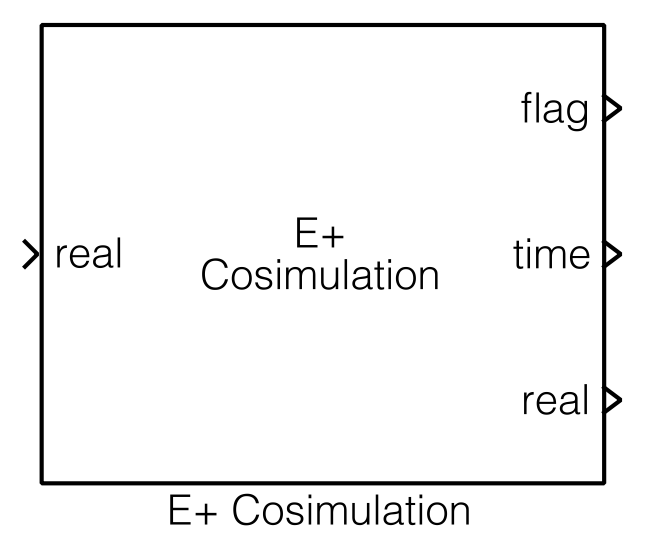
\includegraphics[width=.3\linewidth]{graphics/epblock.png}
\caption{\label{fig:epblock}\emph{E+ Cosimulation} Block.}
\end{figure}
When the Simulink simulation starts, EnergyPlus is also started and will run in
parallel with Simulink.  They then exchange inputs and outputs via socket
communication.  When the simulation terminates, EnergyPlus will exit
automatically.

\emph{E+ Cosimulation} block has one input port and three
output ports:
\begin{itemize}
\item The input is the real vector input to EnergyPlus.
\item The first output (\emph{flag}) is the status of EnergyPlus.
It is 0 if everything is normal, 1 if EnergyPlus has stopped its
simulation, and negative if there was an error.  Simulink should
stop the simulation as soon as this flag is non-zero.
\item The second output (\emph{time}) is the current simulation
time of EnergyPlus, in seconds.
\item The last output (\emph{real}) is the real vector output
from EnergyPlus.
\end{itemize}
Currently, integer and Boolean inputs and outputs are not supported.

Figure \ref{fig:simblock-dlg} shows the parameter dialog box of the
\emph{E+ Cosimulation} block.  These parameters are similar
to the arguments of the function \verb+mlepCreate+ or the
properties of the class \verb+mlepProcess+.  In addition, the
number of real output variables must be specified (this is required by
Simulink).
\begin{figure}[tb]
\centering
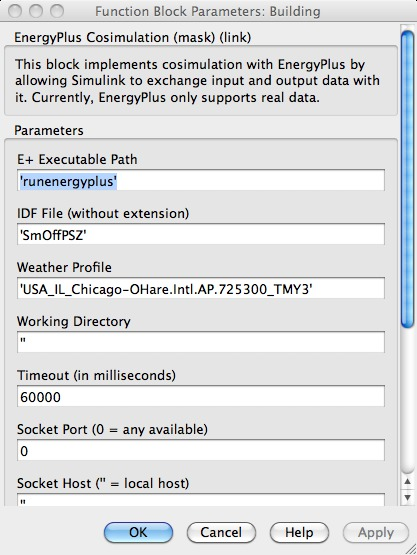
\includegraphics[width=.5\linewidth]{graphics/slblockdlg.jpg}
\caption{\label{fig:simblock-dlg}Parameter dialog of \emph{E+ Cosimulation} Block.}
\end{figure}

\emph{E+ Cosimulation} is a discrete-time block, so either
its time-step is set to a positive value or the Simulink model is
discrete-time.


\section{Examples}
\label{sec:examples}

\MLEP provides an example in which a building and HVAC model is
simulated by EnergyPlus and a controller implemented in Simulink
computes zone temperature set-points.  This example is a
reimplementation of a similar example in the BCVTB distribution.

Figure \ref{fig:example-sl} illustrates a Simulink model that
implements this control system and a plotting window showing the
simulation results.  In the plot are the temperature set-points, the
outdoor dry bulb temperature and the zone temperature for three days,
with a 15-minute time-step.
\begin{figure}[tb]
\centering
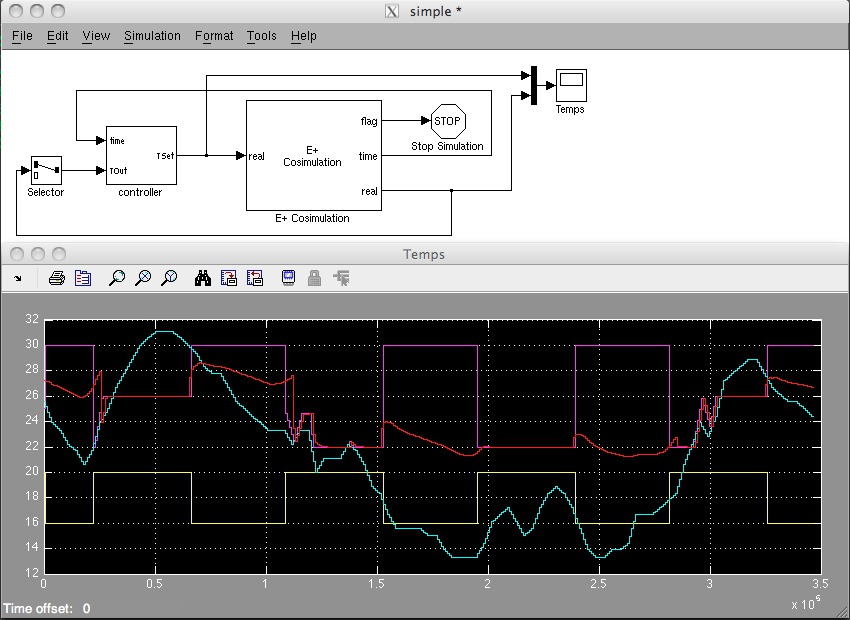
\includegraphics[width=.8\linewidth]{graphics/simulink.jpg}
\caption{\label{fig:example-sl}Simulink model simulation result.}
\end{figure}

The same control system can be implemented in plain Matlab code
instead of Simulink, using the \verb+mlepProcess+ class.
Figure \ref{fig:example-ml} shows the plots of simulation results
computed by this Matlab script, which are the same as those in Figure
\ref{fig:example-sl}.
\begin{figure}[tb]
\centering
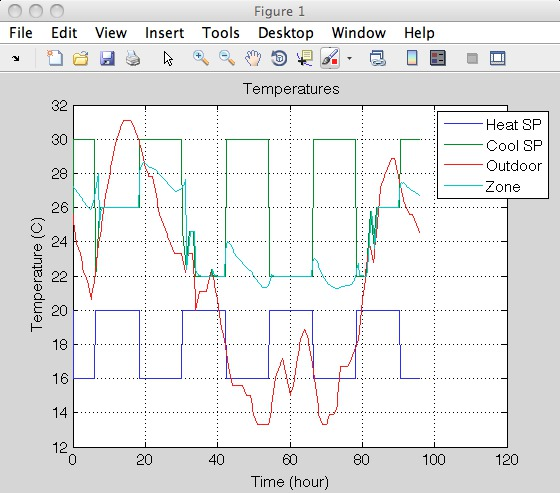
\includegraphics[width=.6\linewidth]{graphics/mlfigure.jpg}
\caption{\label{fig:example-ml}Matlab script simulation result.}
\end{figure}

All Matlab and Simulink example files are located in the sub-directory
\texttt{examples} of the \MLEP distribution.


\bibliographystyle{ieeetr}
\bibliography{mlep_report}

\clearpage
\appendix

\section{\MLEP License}
\label{sec:license}

\MLEP is open-source software.
You are free to use it however you like.
You may redistribute it.
You may modify it to suit your need.

If you redistribute \MLEP or derive your work from \MLEP, you should
give credit to the authors by including their names in your work and/or citing this report.
You are encouraged to share any derivative work.

\paragraph{Disclaimer:}
\MLEP IS DISTRIBUTED WITHOUT ANY WARRANTY.  THE AUTHORS
MAKE NO EXPRESS OR IMPLIED WARRANTIES OR CONDITIONS INCLUDING, WITHOUT
LIMITATION, THE WARRANTIES OF MERCHANTABILITY OR FITNESS FOR A
PARTICULAR PURPOSE WITH RESPECT TO THE SOFTWARE.  IN NO EVENT SHALL
THE AUTHORS BE LIABLE FOR ANY SPECIAL, INCIDENTAL, INDIRECT OR
CONSEQUENTIAL DAMAGES CAUSED BY USING THE SOFTWARE.

\end{document}



%%% Local Variables: 
%%% mode: latex
%%% TeX-master: t
%%% End: 
